\documentclass[12pt]{scrartcl}

 

\usepackage[utf8]{inputenc}

\usepackage[T1]{fontenc}

\usepackage{lmodern}

\usepackage[ngerman]{babel}

\usepackage{amsmath}

\usepackage{graphicx}


 

\title{Versuch E45\\ RCL und RC Schwingkreis}

\author{Frederik Strothmann, Henrik Jürgens}

\date{\today}


\begin{document}


 %deckblatt erstellen

\maketitle
\newpage
\tableofcontents
\newpage

%einleitung zu dem experiment

\section{Einleitung}

In diesem Versuch sollen die Eigenschaften einfacher elektrischer Stromkreise, die aus ”passiven“ Elementen wie
Widerständen, Kondensatoren und Spulen aufgebaut sind, untersucht werden. Weiterhin soll das RC-Glied und das
RL-Glied als Filter für Frequenzen benutzt werden. Je nach Schaltung entsteht ein Hoch– bzw. Tiefpass. Schließlich sollen die gedämpfte elektrische Schwingung bei einem RCL-Kreis und die erzwungene Schwingung
in einem LC-Schwingkreis mit Hilfe des Oszillographen untersucht werden. Bei den Untersuchungen werden kommerzielle elektrische Geräte wie Funktionsgenerator, Digitalmultimeter und ein Oszillograph eingesetzt, so dass am Ende der Versuche eine gewisse Vertrautheit mit der Bedienung der Geräte erwartet wird. Die Versuche werden mit dem Leybold-Stecksystem aufgebaut. Im Einzelnen gliedern sich die Experimente in folgende Teile:
\newline
1)
Messungen an Spannungsteilern
\newline
2)
Messung der Entladekurve eines Kondensators mit Hilfe des Oszillographen
\newline
3)
Messung der Eigenschaften eines RC- oder RL-Filters (Hoch-, Tief- und Bandpass)
\newline
4)
Untersuchung der ungedämpften und der gedämpften elektrischen Schwingung bei einem RCL-Kreis mit Hilfe des Oszillographen
%versuchsaufbau mit skizze

\section{Versuchsaufbau}


\section{Aufgabe 1: Kennenlernen der Geräte}
\subsection{Praktische Durchführung} 
(Wenn Sie sich mit den Geräten bereits gut auskennen, können Sie diese ersten Versuchsteile überspringen.)
\begin{enumerate}
\item
Verbinden Sie das Netzteil mit dem Digitalmultimeter, stellen Sie verschiedene Spannungen ein und messen Sie diese nach. Vergleichen Sie die Anzeigen am Netzteil und am Multimeter. Bauen Sie sich ein symmetrisches Netzteil aus den beiden Ausgängen des Netzgerätes. Messen Sie bezogen auf die mittlere Buchse (GND) die Spannungen zur linken bzw. rechten Buchse. Messen Sie die Gesamtspannung Schließen Sie einen Widerstand (100 $\Omega$, 2 Watt) an das Netzteil an und messen Sie mit dem Multimeter den Strom. Vergleichen Sie die Anzeigen am Netzteil und am Multimeter. Um den Widerstand nicht zu überlasten, stellen Sie die Spannung niemals größer als 14 V ein!
\item
Messen Sie verschiedene Widerstände (100$\Omega$, 10 k$\Omega$, 1 M$\Omega$) mit dem Multimeter nach. Nehmen Sie einen
einstellbaren Widerstand (Potentiometer, 100 k
$\Omega$) und messen Sie in verschiedenen Stellungen den Widerstand.
\item
Verbinden Sie den Funktionsgenerator über ein BNC-Kabel mit den Oszilloskop. Stellen Sie
den Funktionsgenerator auf eine Frequenz von 1 kHz und eine Amplitude von ca. 1 V. Beobachten Sie die Darstellung am Oszilloskop. Sollten Sie Schwierigkeiten haben, ein vernünftiges Bild zu bekomen, hilft Ihnen bei unseren Digitaloszilloskopen die Taste ”Autoset“ weiter. Stellen Sie verschiedene Funktionen ein (Sinus, Dreieck, Rechteck). Beobachten Sie die Wirkung der Einstellung ”Offset“ (Verschiebung um eine konstante Gleichspannung) oder ”duty cycle“ (Impuls-Pausen-Verhältnis). Ändern Sie die Frequenz am Generator und passen Sie die Einstellung am Oszilloskop (x-Achse, Time) von
Hand an (die Autoset-Taste sollte nur in Ausnahmefällen betätigt werden. Der erfahrene Benutzer bekommt von Hand oft sinnvollere Darstellungen). Ändern Sie die Amplitude am Generator und passen Sie die Einstellung am Oszilloskop (y-Achse, Ch1) von Hand an. Machen Sie sich mit den Funktionen Measure und Cursor
vertraut, die Ihnen ein schnelles und einfaches Messen wichtiger Größen ermöglichen.
\item
Für den folgenden Versuchsteil müssen Sie sich mit Ihrer Nachbargruppe zusammentun, weil zwei Funktionsgenaratoren benötigt werden. Schließen Sie den einen an Kanal 1 und den anderen an Kanal 2 eines Oszilloskops an. Stellen Sie das Oszilloskop in den ”x-y-Modus“. Auf Kanal 1 geben Sie eine Sinusspannung mit einer Frequenz von genau 50 Hz, auf Kanal 2 das gleiche mit genau 100 Hz. Beobachten Sie die Darstellung, wenn Sie die Frequenzen minimal ändern. Aus den sogenannten
LISSAJOUS-Ellipsen können Sie den Phasenwinkel zwischen den beiden Schwingungen genau bestimmen. Beobachten Sie, was bei anderen einfachen Frequenzverhältnissen $\frac{f_1}{f_2}$ passiert.
\item
Stellen Sie den Funktionsgenerator auf Sinus, 50 Hz, Amplitude einige Volt. Messen Sie die Amplitude am Oszilloskop. Schließen Sie ein Digitalvoltmeter (Bereich AC V) an und vergleichen Sie den Anzeigewert mit dem des Oszilloskops. Wiederholen Sie die Messungen bei 500 Hz, 5kHz und 50 kHz. Was fällt auf?
\end{enumerate}
\subsection{Diskussion}
In dieser Aufgabe haben wir uns mit den Geräten vertraut gemacht, da wir diese zum Teil nicht kannten.
\section{Aufgabe 2: Einfache Schaltungen mit Widerständen und Kondensatoren}
\subsection{Praktische Durchführung} 
\begin{enumerate}
\item
Bauen Sie sich mit zwei Widerständen einen Spannungsteiler (s. Schaltplan). Messen Sie mit dem DMM die Knotenspannung U2 und vergleichen Sie mit dem Theoriewert. Verwenden Sie zunächst zwei Widerstände aus dem k$\Omega$-Bereich und später zwei von 1 M$\Omega$. Was fällt auf? Erklären Sie die Abweichungen vom Theoriewert. Beachten Sie den Innenwiderstand des DMM (typ. 10 M
$\Omega$)
%Abbildung 17:Schaltplan Spannungsteiler
\begin{figure}[htbp] 
  \centering
    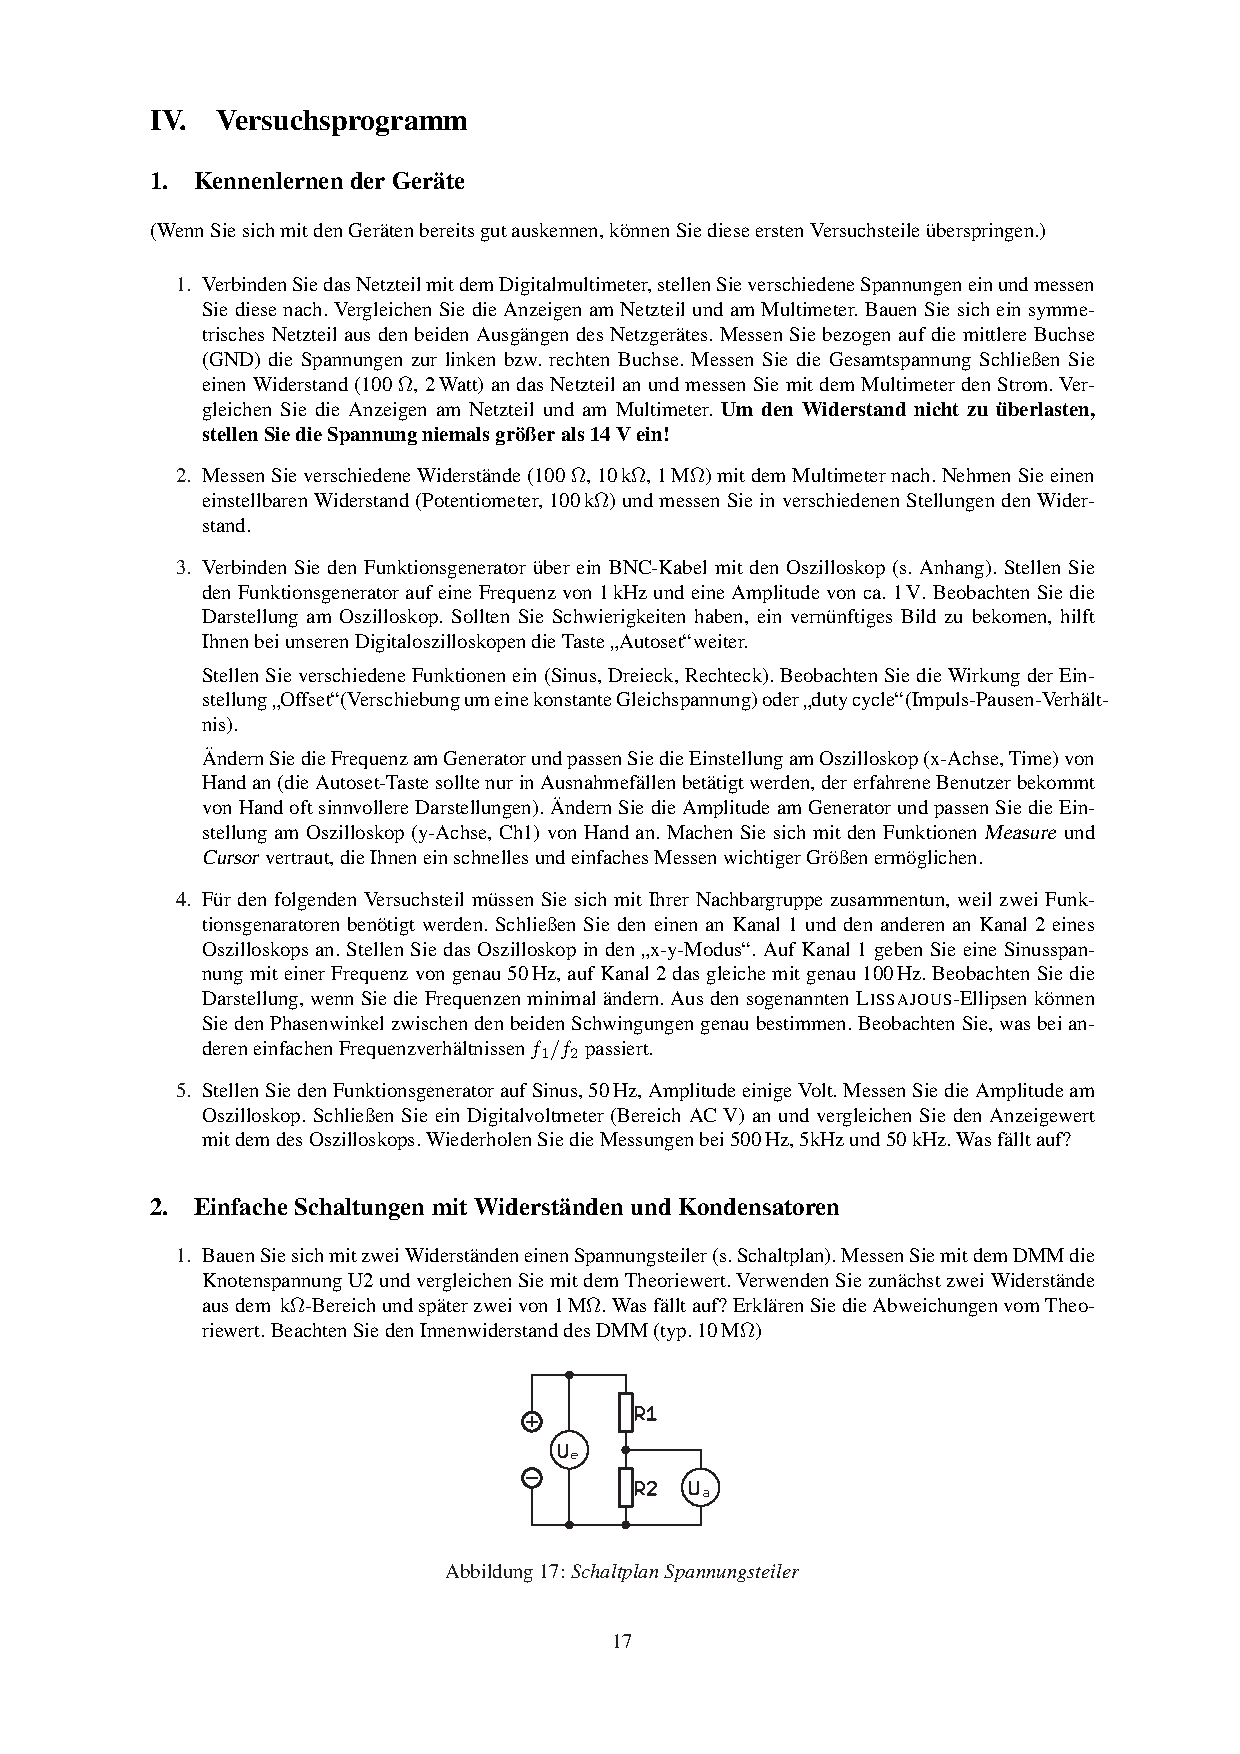
\includegraphics[trim = 30mm 35mm 1mm 228mm, clip, scale = 1]{spannungsteiler.pdf}
  	\caption[Skizze der Schaltung für einen Spannungsteiler]{Skizze der Schaltung für einen Spannungsteiler\footnotemark}
  \label{fig:spannungsteiler}
\end{figure}
\footnotetext{Abbildung entnommen von http://www.atlas.uni-wuppertal.de/~kind/E45neu0910.pdf Seite 17 am 22.08.2014}

\item
Verbinden Sie den Funktionsgenerator (Rechteck, 100 Hz) über einen Widerstand (10 k
$\Omega$) mit einem Kondensator (100 nF). Messen Sie die Spannung $U_a$ Über dem Kondensator mit dem Oszilloskop. Bestimmen
Sie die Halbwertszeit; dabei hilft Ihnen die Cursor-Funktion des Oszilloskops. Vergleichen Sie mit dem Theoriewert $\ln(2)RC$.
%Abbildung 18: Schaltplan zur Entladekurve (Oszilloskopmesung)
\begin{figure}[htbp] 
  \centering
    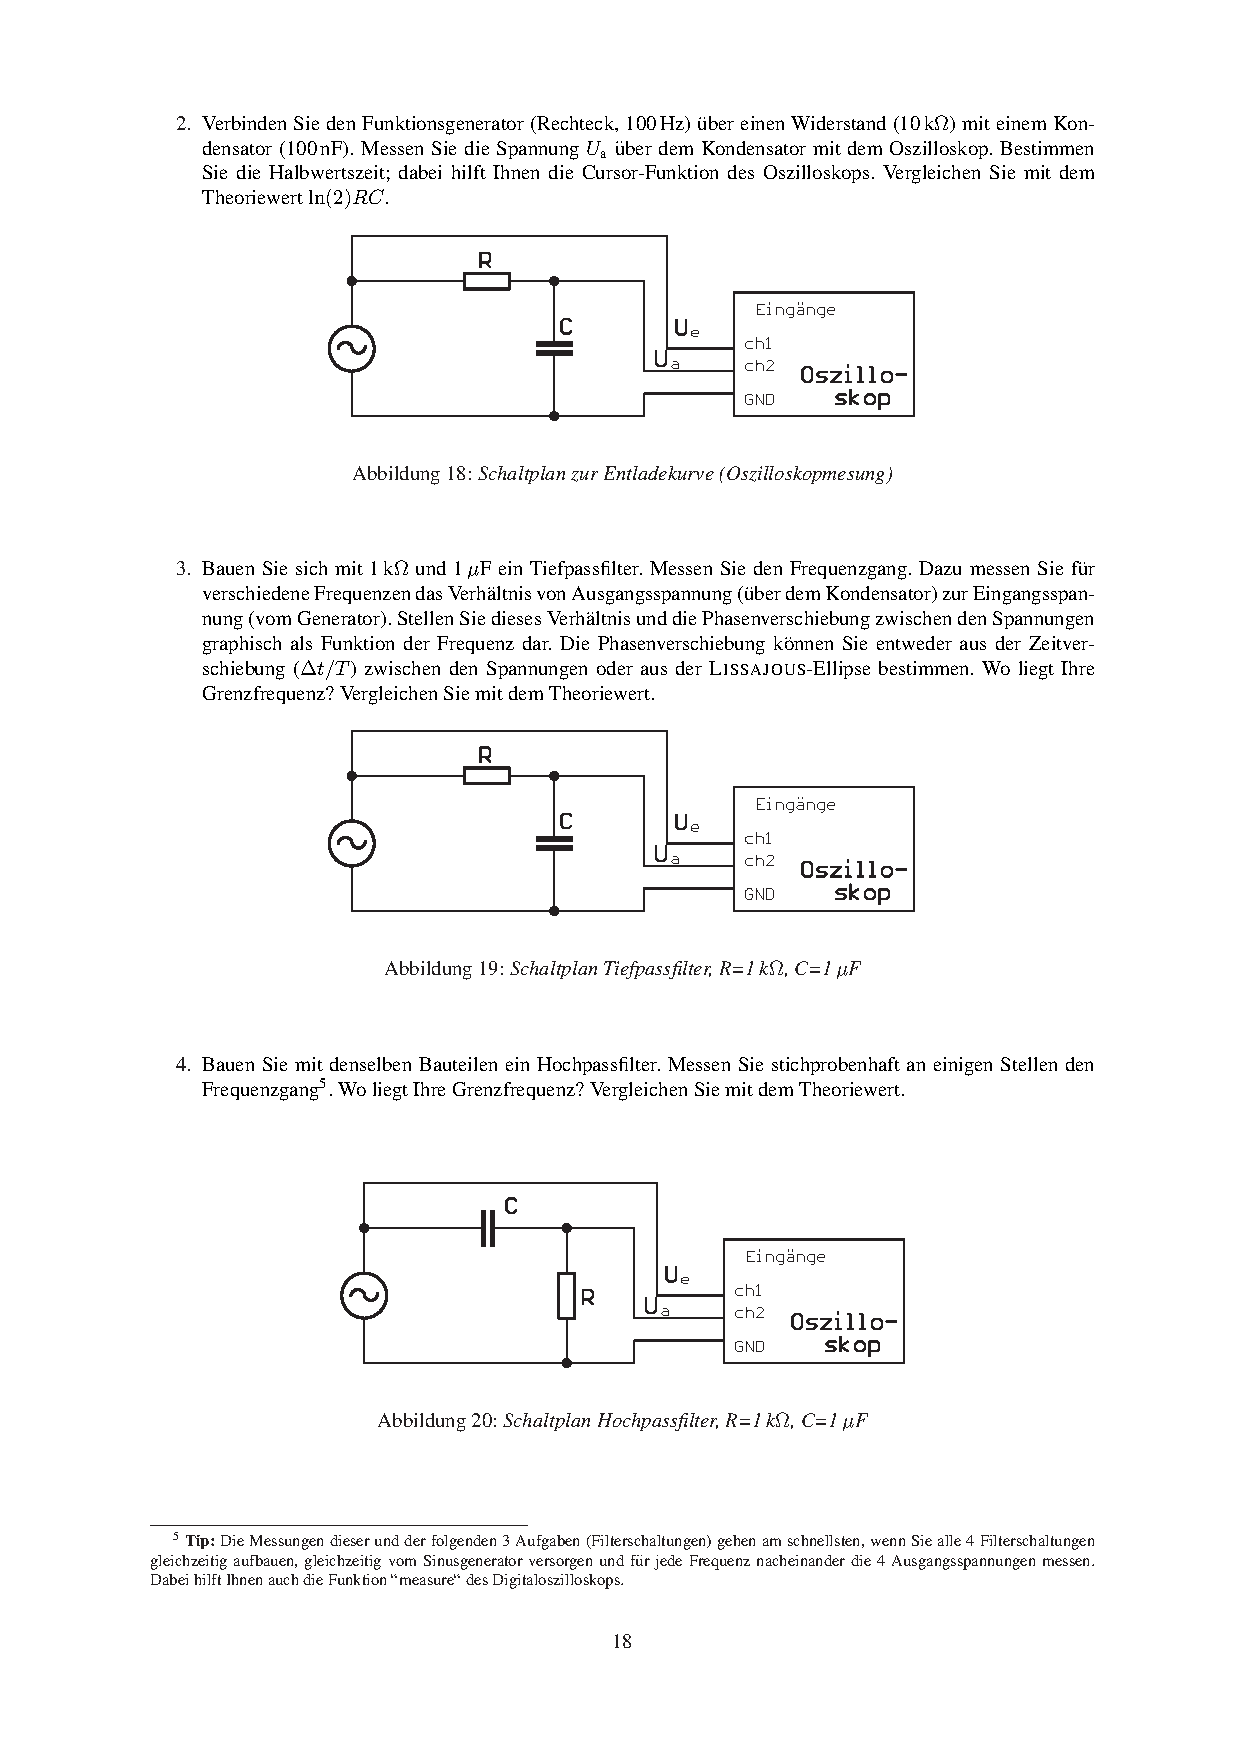
\includegraphics[trim = 1mm 225mm 1mm 37mm, clip, scale = 1]{tiefpass.pdf}
  	\caption[Skizze der Schaltung für einen Tiefpass]{Skizze der Schaltung für einen Tiefpass\footnotemark}
  \label{fig:Tiefpass_2}
\end{figure}
\footnotetext{Abbildung entnommen von http://www.atlas.uni-wuppertal.de/~kind/E45neu0910.pdf Seite 18 am 22.08.2014}

\item
Bauen Sie sich mit 1 k$\Omega$ und 1
$\mu$F ein Tiefpassfilter. Messen Sie den Frequenzgang. Dazu messen Sie für
verschiedene Frequenzen das Verhältnis von Ausgangsspannung (über dem Kondensator) zur Eingangsspannung (vom Generator). Stellen Sie dieses Verhältnis und die Phasenverschiebung zwischen den Spannungen graphisch als Funktion der Frequenz dar. Die Phasenverschiebung können Sie entweder aus der Zeitverschiebung ($\frac{\Delta t}{T}$) zwischen den Spannungen oder aus der LISSAJOUS-Ellipse bestimmen. Wo liegt Ihre Grenzfrequenz? Vergleichen Sie mit dem Theoriewert.
%Abbildung 19: Schaltplan Tiefpassfilter, R=1 k$\Omega$, C=1$\mu$F
\begin{figure}[htbp] 
  \centering
    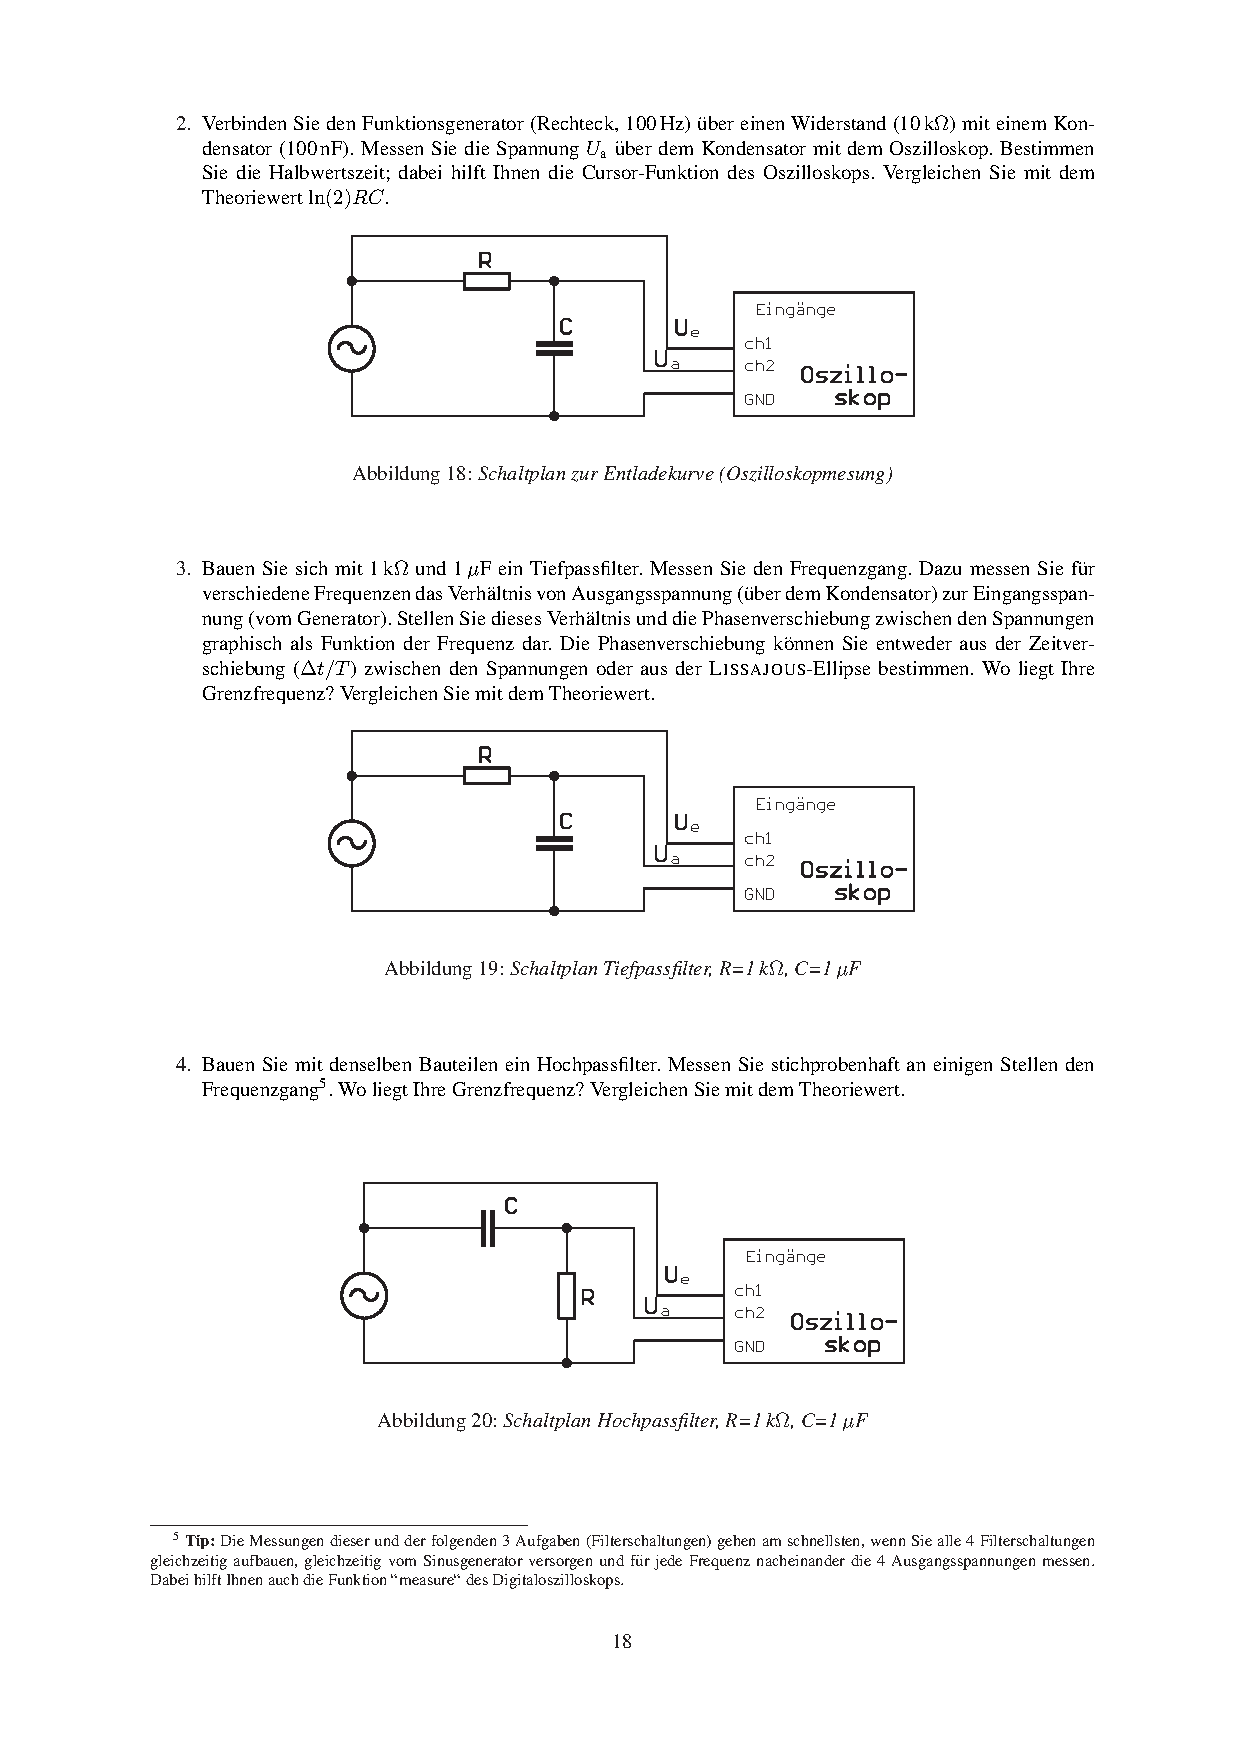
\includegraphics[trim = 1mm 225mm 1mm 37mm, clip, scale = 1]{tiefpass.pdf}
  	\caption[Skizze der Schaltung für einen Tiefpass]{Skizze der Schaltung für einen Tiefpass\footnotemark}
  \label{fig:Tiefpass_2}
\end{figure}
\newpage
\footnotetext{Abbildung entnommen von http://www.atlas.uni-wuppertal.de/~kind/E45neu0910.pdf Seite 18 am 22.08.2014}
\item
Bauen Sie mit denselben Bauteilen ein Hochpassfilter. Messen Sie stichprobenhaft an einigen Stellen den Frequenzgang (Tipp: Die Messungen dieser und der folgenden 3 Aufgaben (Filterschaltungen) gehen am schnellsten, wenn Sie alle 4 Filterschaltungen
gleichzeitig aufbauen, gleichzeitig vom Sinusgenerator versorgen und für jede Frequenz nacheinander die 4 Ausgangsspannungen messen.
Dabei hilft Ihnen auch die Funktion “measure“ des Digitaloszilloskops.). Wo liegt Ihre Grenzfrequenz? Vergleichen Sie mit dem Theoriewert.
%Abbildung 20: Schaltplan Hochpassfilter, R=1 k$\Omega$, C=1$\mu$F
\begin{figure}[htbp] 
  \centering
    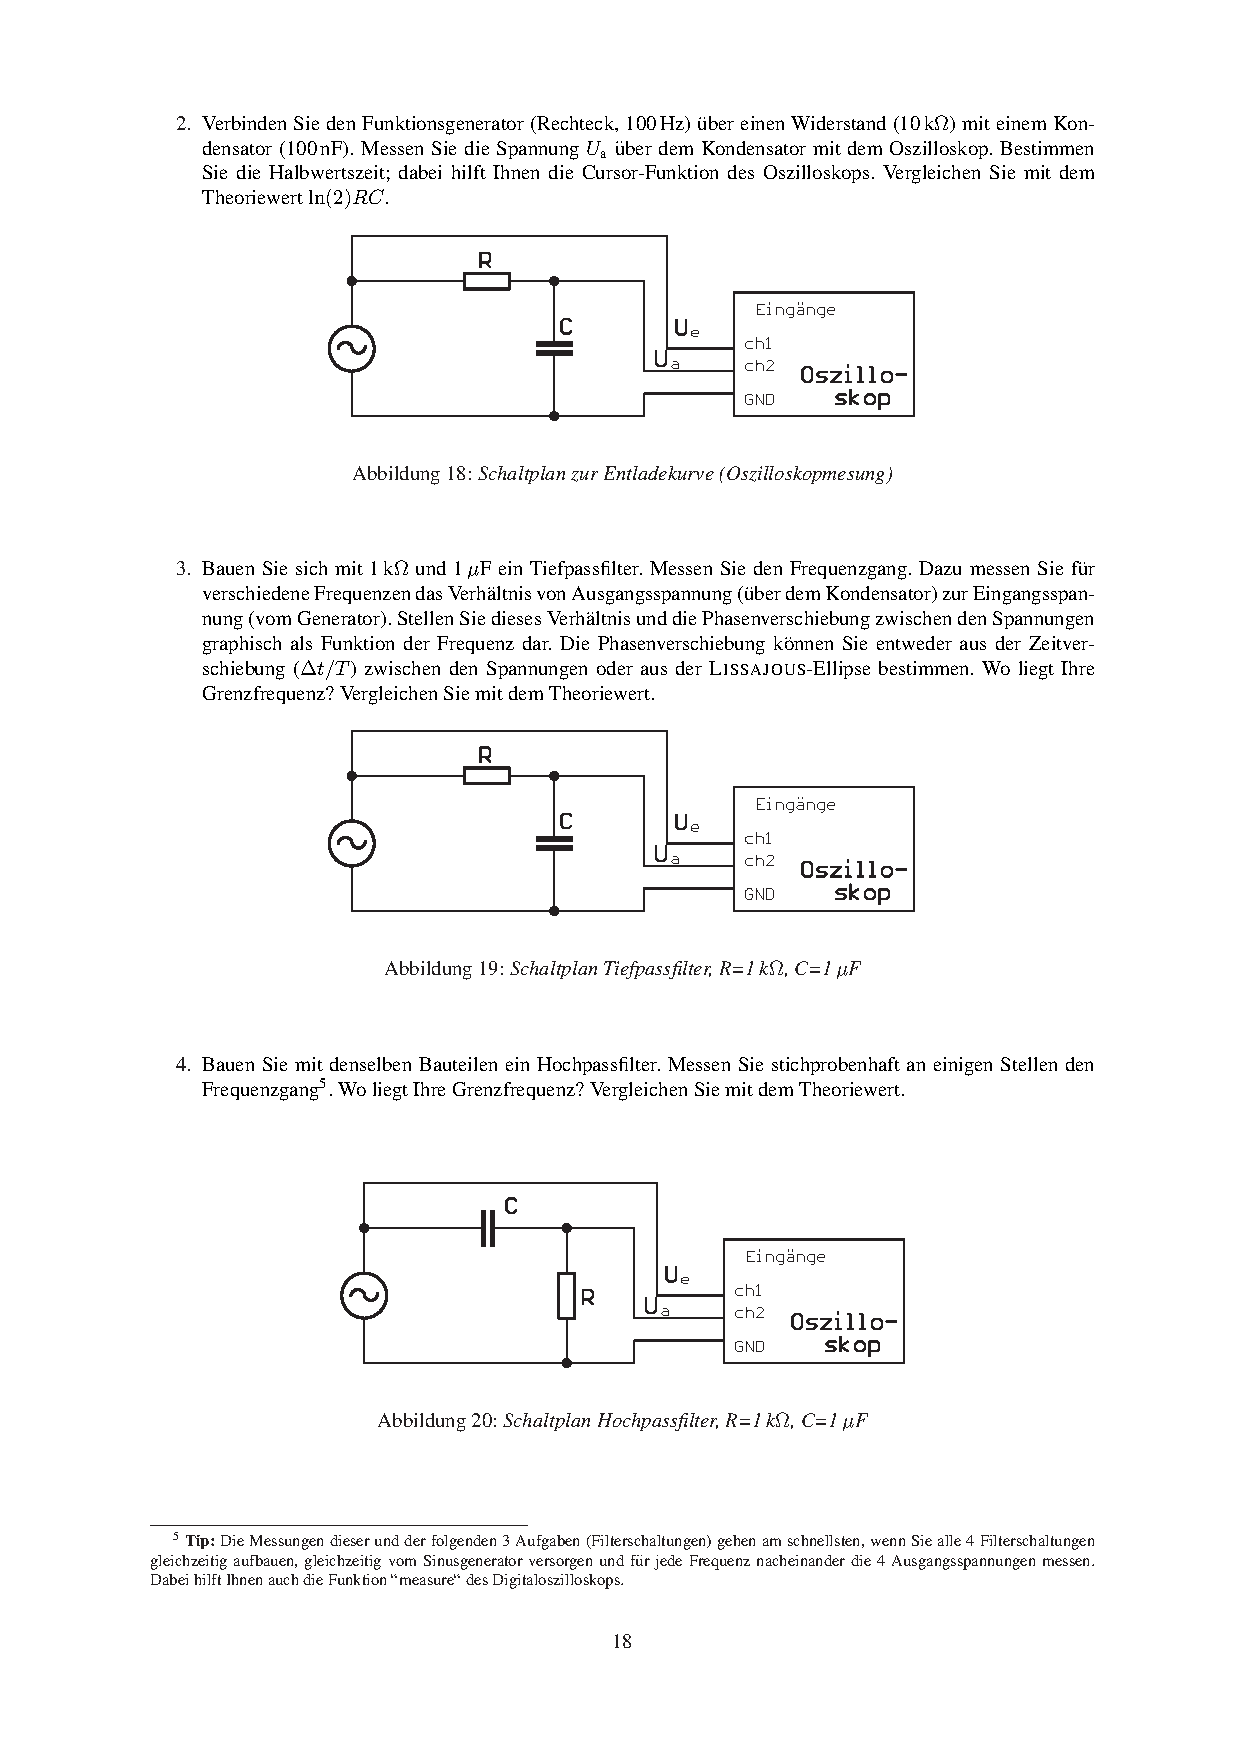
\includegraphics[trim = 20mm 60mm 1mm 190mm, clip, scale = 1]{tiefpass.pdf}
  	\caption[Skizze der Schaltung für einen Hockpass]{Skizze der Schaltung für einen Hochpass\footnotemark}
  \label{fig:Hochpass}
\end{figure}
\footnotetext{Abbildung entnommen von http://www.atlas.uni-wuppertal.de/~kind/E45neu0910.pdf Seite 18 am 22.08.2014}
\item
Bauen Sie sich mit weiteren Bauelementen einen Bandpaßfilter und untersuchen Sie an einigen Stellen den Frequenzgang (Graphen!). Wo liegen die Grenzfrequenzen? Vergleichen Sie mit dem Theoriewert.
%Abbildung 21: Schaltplan Bandpassfilter, R1=1 k$\Omega$, C1=1$\mu$F, R2=10 k$\Omega$, C2=1nF
\begin{figure}[htbp] 
  \centering
    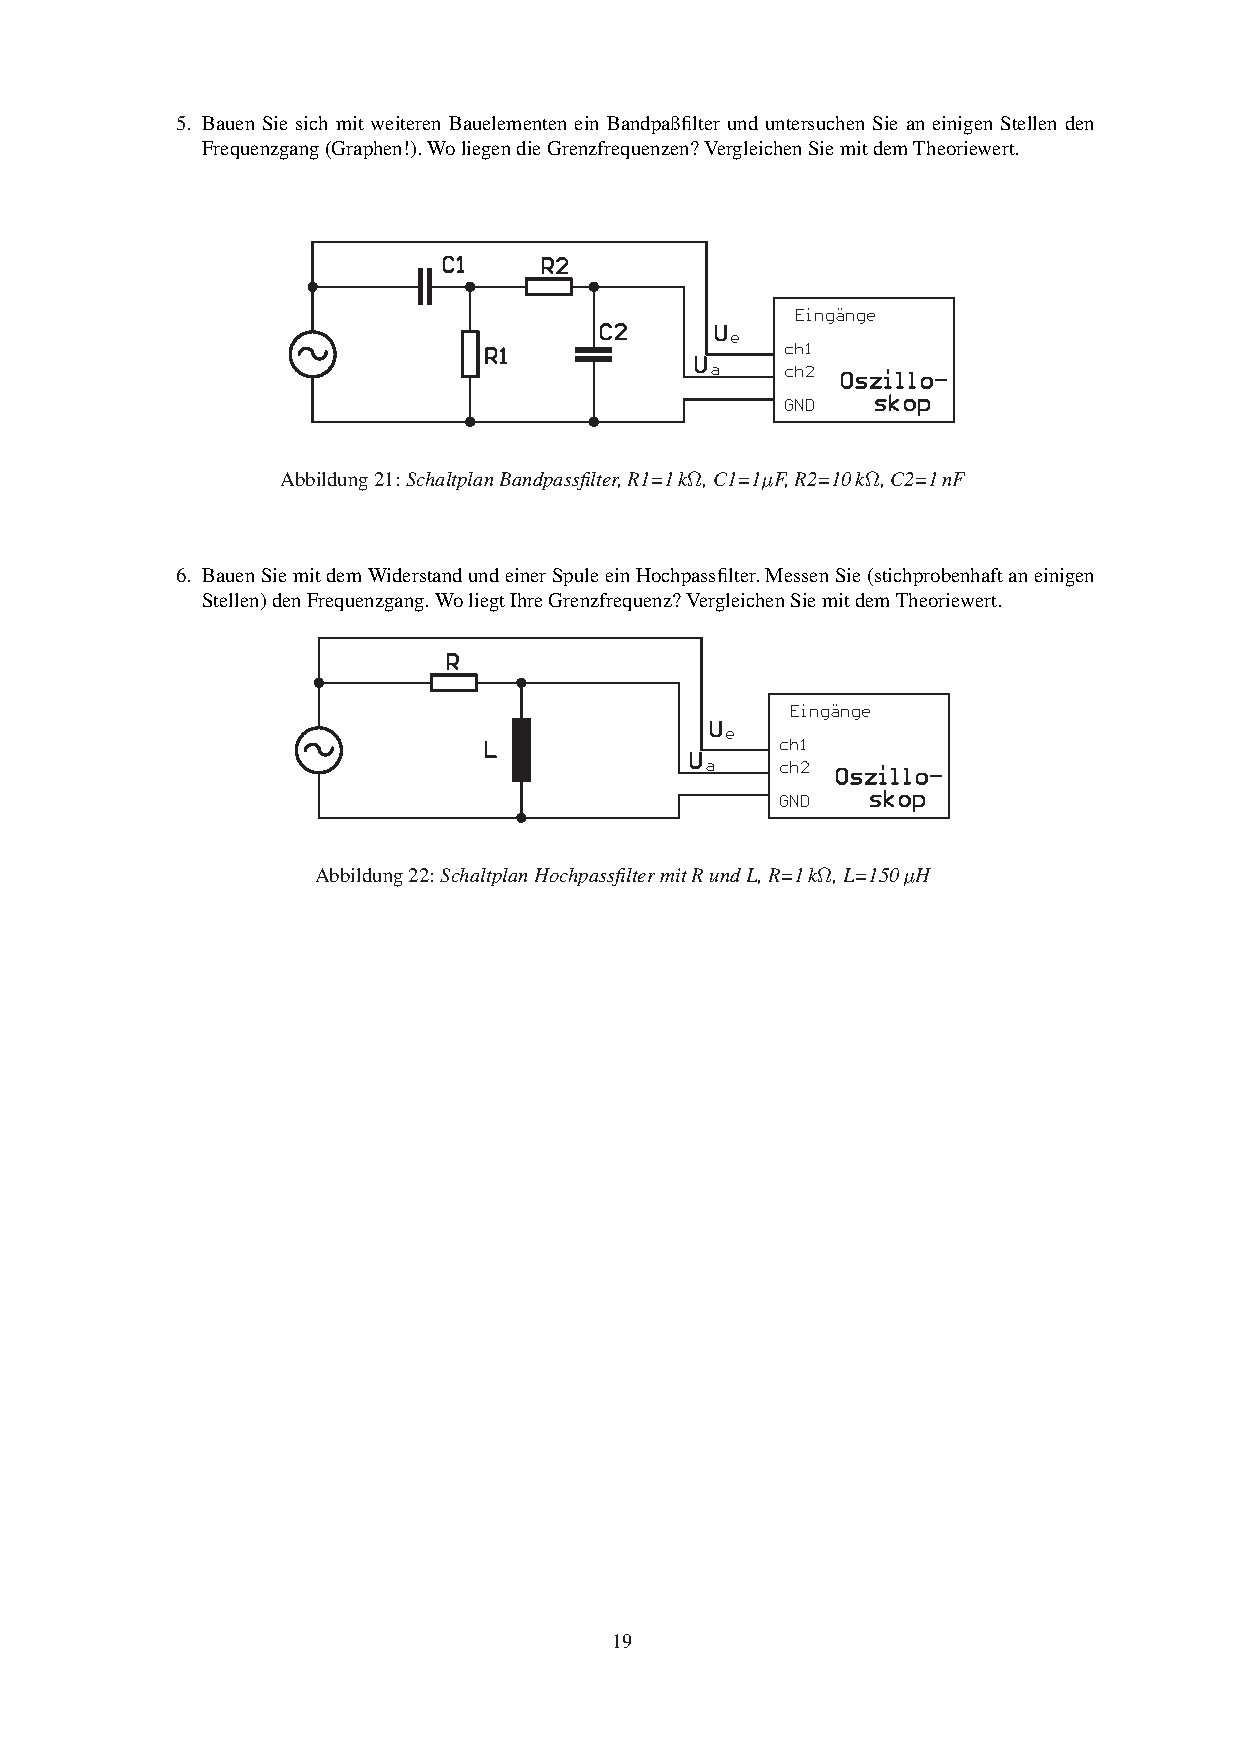
\includegraphics[trim = 20mm 220mm 1mm 30mm, clip, scale = 1]{bandpass_hochpass.pdf}
  	\caption[Skizze der Schaltung für einen Bandpass]{Skizze der Schaltung für einen Bandpass\footnotemark}
  \label{fig:Bandpass}
\end{figure}
\newpage
\footnotetext{Abbildung entnommen von http://www.atlas.uni-wuppertal.de/~kind/E45neu0910.pdf Seite 19 am 22.08.2014}
\item
Bauen Sie mit dem Widerstand und einer Spule ein Hochpassfilter. Messen Sie (stichprobenhaft an einigen Stellen) den Frequenzgang. Wo liegt Ihre Grenzfrequenz? Vergleichen Sie mit dem Theoriewert.
%Abbildung 22: Schaltplan Hochpassfilter mit R und L, R=1 k$\Omega$, L=150$\mu$H
\begin{figure}[htbp] 
  \centering
    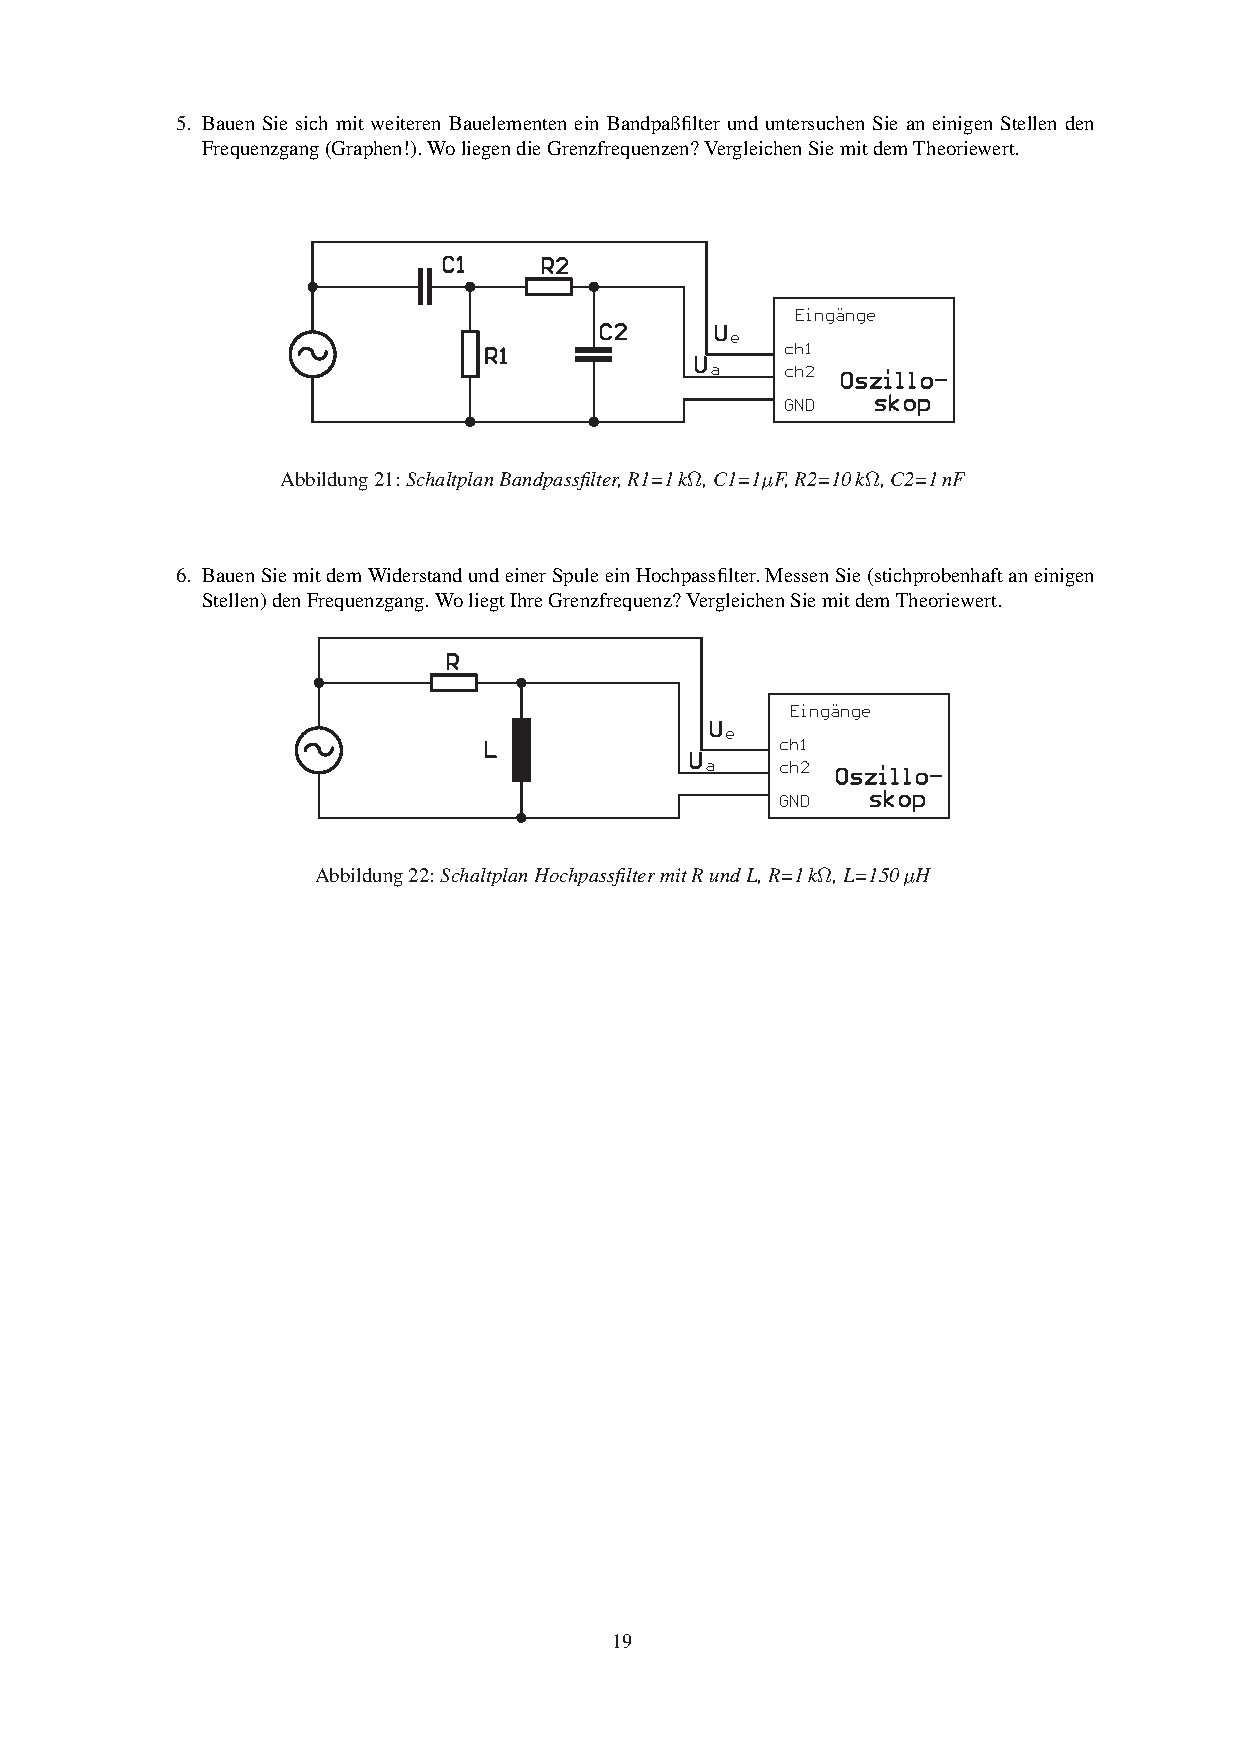
\includegraphics[trim = 20mm 155mm 1mm 105mm, clip, scale = 1]{bandpass_hochpass.pdf}
  	\caption[Skizze der Schaltung für einen Hochpass, mit einer Spule]{Skizze der Schaltung für einen Hochpass, mit einer Spule\footnotemark}
  \label{fig:Hochpass_spule}
\end{figure}
\footnotetext{Abbildung entnommen von http://www.atlas.uni-wuppertal.de/~kind/E45neu0910.pdf Seite 19 am 22.08.2014}

\end{enumerate}
\subsection{Theoretische Durchführung}
\begin{enumerate}
\item
Reduzierter Widerstand:
\begin{align}
R_L = \frac{R_i R_2}{R_i + R_2}
\end{align}
$R_i$ der Innenwiderstand des Messgerätes,
$R_1$ und $R_2$ die beiden in Reihe geschalteten Widerstände.
Fehler $R_L$:
\begin{align}
\sigma_{R_L} = \sqrt{
\left(\frac{R_i(R_i+R_2)-R_i R_2}{(R_i + R_2)^2}\sigma_{R_2}\right)+
\left(\frac{R_2(R_i+R_2)-R_i R_2}{(R_i + R_2)^2}\sigma_{R_i}\right)}
\end{align}
Spannungsteiler:
\begin{align}
U_a = U_e \frac{R_L}{R_L + R_1}
\end{align}
Fehler Spannungsteiler:
\begin{align}
\sigma_{U_a} = \sqrt{
\left(\frac{R_L}{R_L + R_1}\sigma_{U_e}\right)^2+
\left(U_e \frac{R_1}{(R_L + R_1)^2}\sigma_{R_L}\right)^2+
\left(U_e \frac{R_L}{(R_L + R_1)^2}\sigma_{R_1}\right)^2}
\end{align}
\item
Die Formel für die Halbwertszeit ist:
\begin{align}
T_{\frac{1}{2}} = \ln(2)RC
\end{align}
Fehler:
\begin{align}
\sigma_{T_{\frac{1}{2}}} = \sqrt{
\left(\ln(2)R\sigma_{C}\right)^2+
\left(\ln(2)C\sigma_{R}\right)^2}
\end{align}
\item
Im folgenden gilt immer:
\begin{align}
\omega = 2\pi f
\end{align}
Fehler:
\begin{align}
\sigma_{\omega} = 2\pi\sigma_f
\end{align}
Die Grenzfrequenz/en in Aufgabe 3,4 und 5 sind:
\begin{align}
\omega_{Gr} = \frac{1}{RC}
\end{align}
Fehler:
\begin{align}
\sigma_{\omega_{Gr}} = \sqrt{
\left(\frac{1}{R^2C}\sigma_R\right)^2+
\left(\frac{1}{RC^2}\sigma_C\right)^2}
\end{align}
\item
Die Grenzfrequenz in Aufgabe 6 ist:
\begin{align}
\omega_{Gr} = \frac{R}{L}
\end{align}
Fehler:
\begin{align}
\sigma_{\omega_{Gr}} = \sqrt{\left(\frac{1}{L}\sigma_R\right)^2+\left(\frac{R}{L^2}\sigma_L\right)^2}
\end{align}

\end{enumerate}
\subsection{Diskussion}
Im ersten Teil dieser Aufgabe sollte die Knotenspannung an einem Spannungsteiler ausgemessen und mit dem Theoriewert verglichen werden. Der erste gemessene Wert liegt im ersten Sigmaintervall des Theoriewertes, der zweite gemessene Wert liegt knapp außerhalb des ersten, aber innerhalb des zweiten Sigmaintervalls des Theoriewertes (das gleiche gilt umgekehrt für die beiden Theoriewerte bezogen auf die Fehler der Messwerte). 
Im zweiten Teil sollte die Halbwertszeit der Entladung des Kondensators in einem RC Tiefpasses bestimmt und mit dem Theoriewert verglichen werden. Der gemessene Wert lag erst im zweiten Sigmaintervall des Theoriewertes (sowie der Theoriewert erst im zweiten Sigmaintervall des Messwertes). Das liegt einerseits daran, dass wir den Fehler auf Widerstand und Kondensator nicht kannten (schätzen mussten) und andererseits den Fehler, der durch den Innenwiderstand des Spannungsmessgerätes bei abfallender Spannung entsteht, nicht berücksichtigt haben.
Im dritten bis sechsten Teil sollten die Grenzfrequenzen von Hoch-, Tief- und Bandpass bestimmt und mit den Theoriewerten verglichen werden. Dabei wurde der Hochpass einerseits aus einem RC-Glied sowie andererseits aus einem RL-Glied geschaltet. Band- und Tiefpass wurden ausschließlich aus RC-Gliedern geschaltet. Im Aufgabenteil drei ergibt sich mit den Messwerten der Nachbargruppe eine Grenzfrequenz, die innerhalb des ersten Sigmaintervalls des Theoriewertes liegt.
Im Aufgabenteil 4 bis 6 haben wir leider den falschen Frequenbereich ausgemessen, da wir $\omega_Gr$ nicht in das am Funktionsgenerator angezegte f umgerechnet haben.
Dies sieht man sehr gut an den Plots
%(\ref plots)
für Aufgabenteil 4 und 6, wodurch diese nicht für den Vergleich mit den Theoriewerten zu gebrauchen sind.
Plot 5 ist zwar sehr ungenau, es lässt sich aber eine der beiden Grenzfrequenzen über einen manuellen Fit ablesen, welche auch relativ nahe an dem Theoriewert liegt, jedoch können wir wegen der großen Ungenauigkeit durch den manuellen Fit keine weiteren Aussagen zur Fehlerbetrachtung in diesem Versuchsteil angeben.
\section{Aufgabe 3: LC-Kreis}
\subsection{Praktische Durchführung}
\subsubsection{Resonanzkurve} 
Nun nehmen wir eine Resonanzkurve auf, also $U_C$ als Funktion der Frequenz. Stellen Sie den Funktionsgenerator wieder auf SINUSsignal. Wir nehmen zunächst einen LC-Parallelresonanzkreis (Bei einem Serien-Resonanzkreis wie in 4. wird der Widerstand (genauer: die Impedanz) im Resonanzfall sehr klein. Dadurch bricht die Ausgangsspannung des Funktionsgenerators (Innenwiderstand 50
$\Omega$) zusammen und die Resonanzerhöhung der Spannung über L oder C ist
nur schlecht zu erkennen. Beim Parallelresonanzkreis wird der Widerstand (die Impedanz) im Resonanzfall sehr groß und man sieht einen deutlichen Resonanzpeak).
%Abbildung 23: Schaltplan LC-Kreis; L=150$\mu$H, C=1$\mu$F, R = 0 oder (für geringe Güte) 10$\Omega$
\begin{figure}[htbp] 
  \centering
    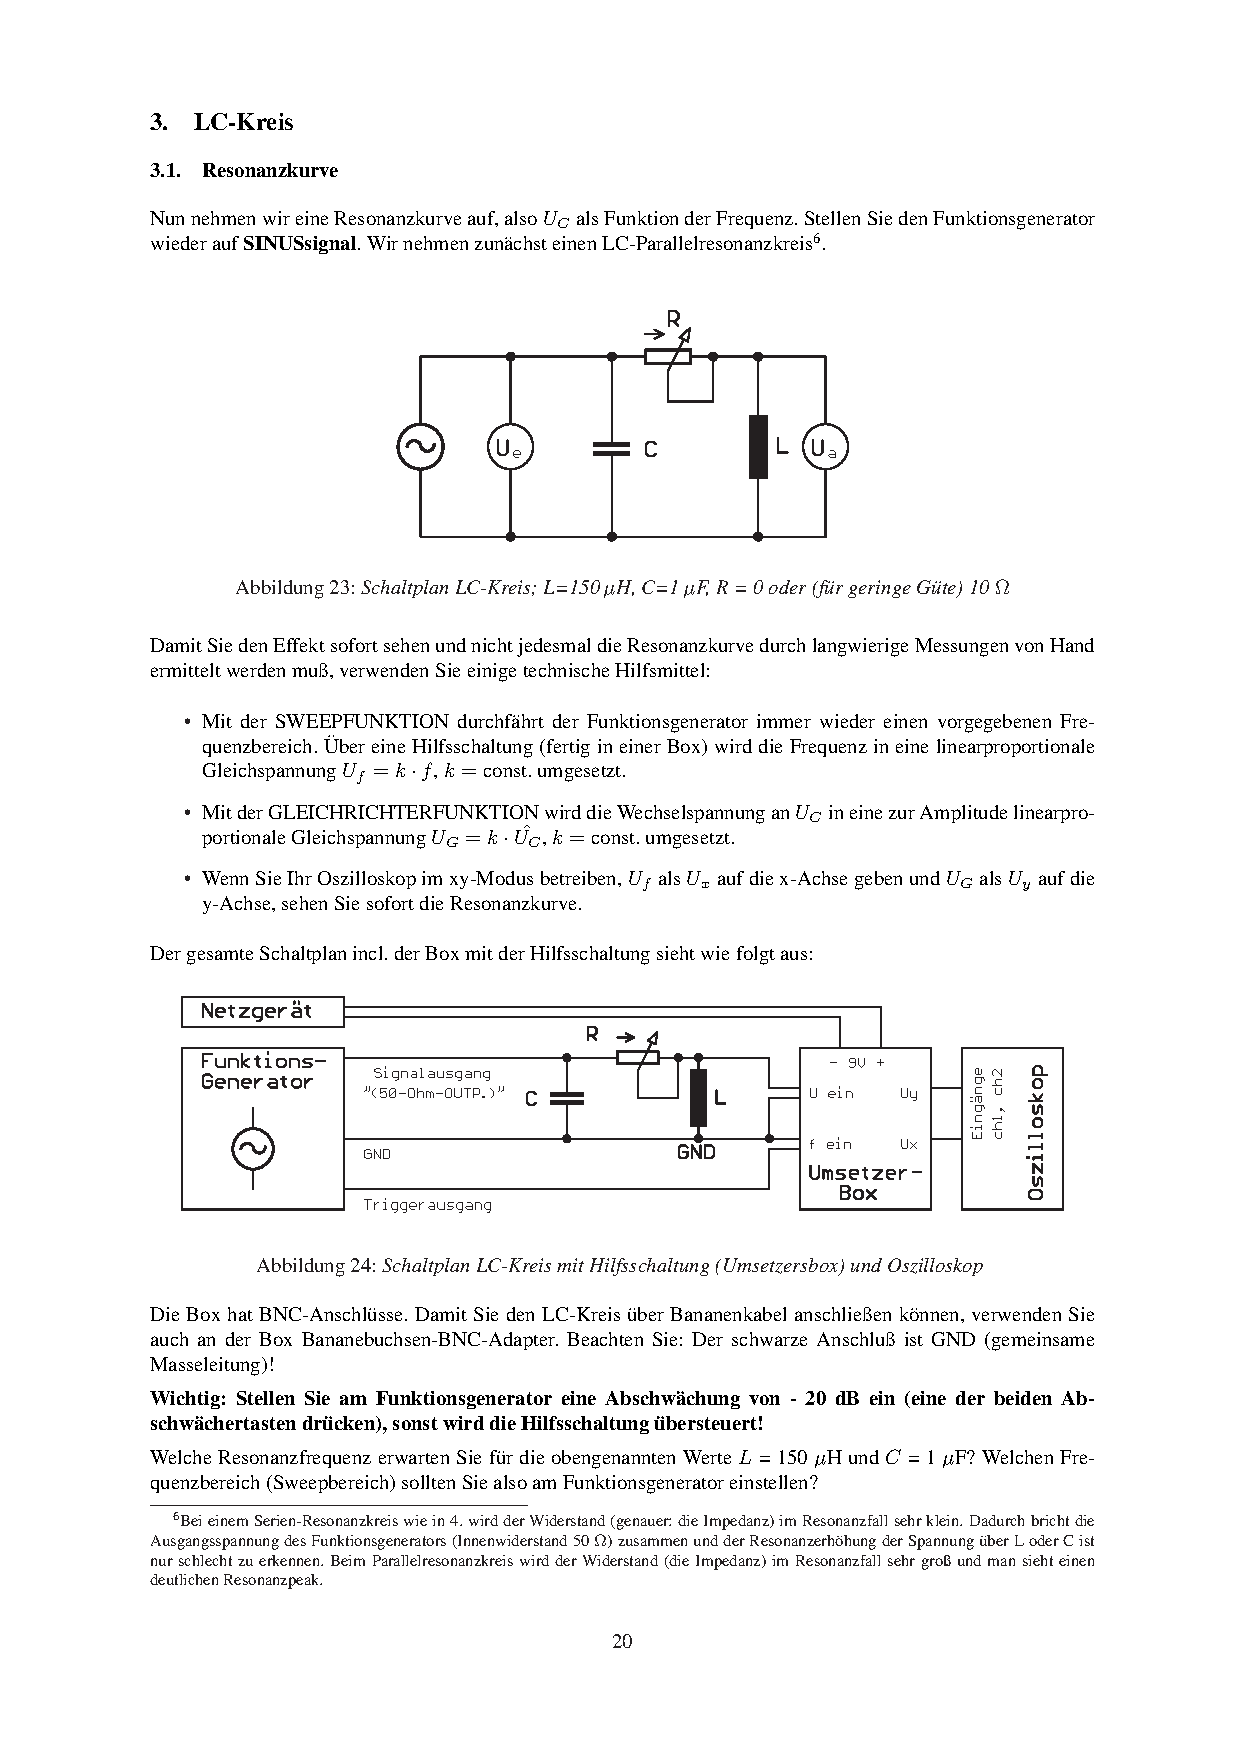
\includegraphics[trim = 20mm 200mm 1mm 50mm, clip, scale = 1]{LC_kreis.pdf}
  	\caption[Skizze der Schaltung für einen LC-Kreis]{Skizze der Schaltung für einen LC-Kreis\footnotemark}
  \label{fig:LC-Kreis}
\end{figure}
\footnotetext{Abbildung entnommen von http://www.atlas.uni-wuppertal.de/~kind/E45neu0910.pdf Seite 20 am 22.08.2014}

Damit Sie den Effekt sofort sehen und nicht jedesmal die Resonanzkurve durch langwierige Messungen von Hand
ermittelt werden muß, verwenden Sie einige technische Hilfsmittel:
\begin{itemize}
\item
Mit der SWEEPFUNKTION durchfährt der Funktionsgenerator immer wieder einen vorgegebenen Frequenzbereich. Über eine Hilfsschaltung (fertig in einer Box) wird die Frequenz in eine linearproportionale
Gleichspannung $U_f$ = $k \cdot f$, $k$ = const. umgesetzt.
\item
Mit der GLEICHRICHTERFUNKTION wird die Wechselspannung an $U_C$ in eine zur Amplitude linearproportionale Gleichspannung $U_G = k \cdot \hat{U_C}$ , $k$ = const. umgesetzt.
\item
Wenn Sie Ihr Oszilloskop im xy-Modus betreiben, $U_f$ als $U_x$
auf die x-Achse geben und $U_G$ als $U_y$ auf die y-Achse, sehen Sie sofort die Resonanzkurve.
\end{itemize}
Der gesamte Schaltplan incl. der Box mit der Hilfsschaltung sieht wie folgt aus:
%Abbildung 24: Schaltplan LC-Kreis mit Hilfsschaltung (Umsetzersbox) und Oszilloskop
\begin{figure}[htbp] 
  \centering
    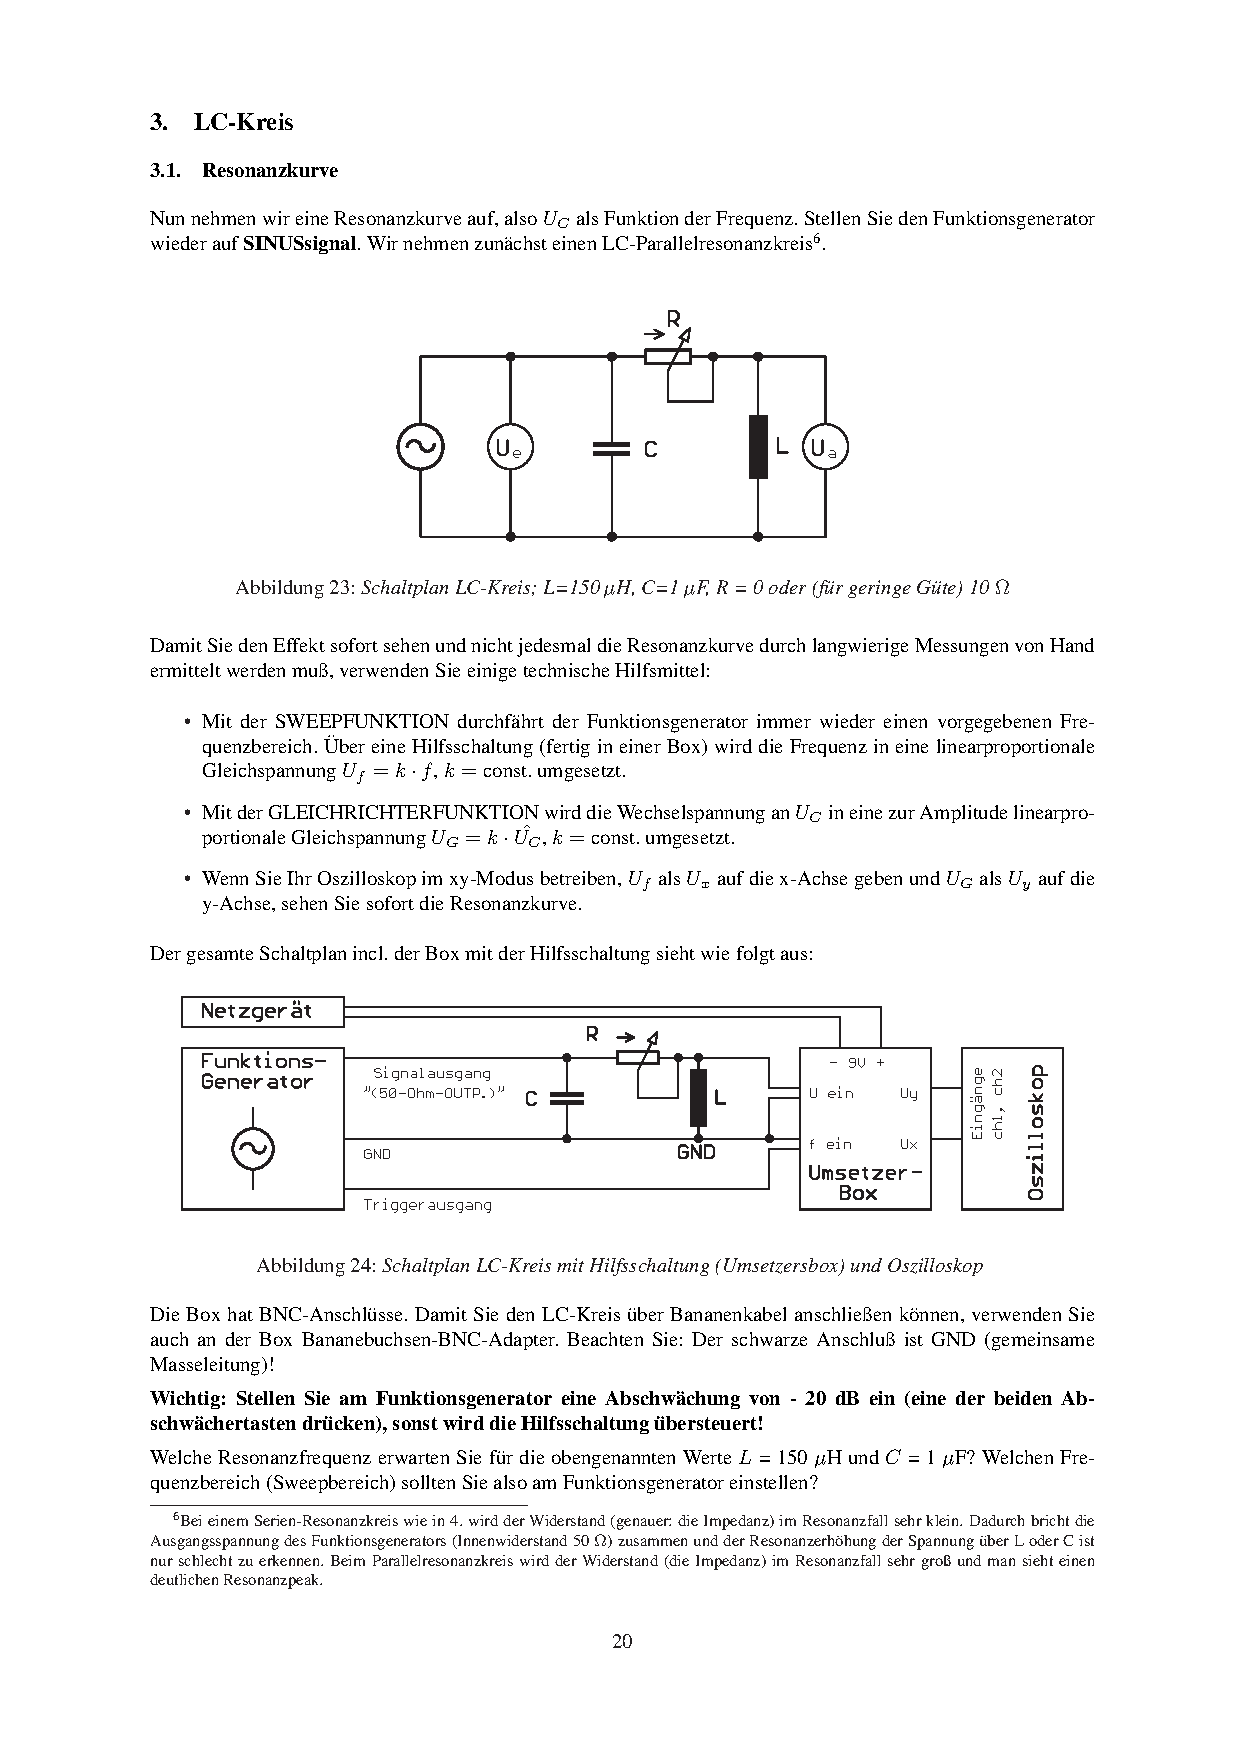
\includegraphics[trim = 20mm 90mm 1mm 165mm, clip, scale = 1]{LC_kreis.pdf}
  	\caption[Skizze der Schaltung für einen LC-Kreis, mit Hilfsschaltung]{Skizze der Schaltung für einen LC-Kreis, mit Hilfsschaltung\footnotemark}
  \label{fig:LC-Kreis_hilfe}
\end{figure}
\footnotetext{Abbildung entnommen von http://www.atlas.uni-wuppertal.de/~kind/E45neu0910.pdf Seite 20 am 22.08.2014}

Die Box hat BNC-Anschlüsse. Damit Sie den LC-Kreis über Bananenkabel anschließen können, verwenden Sie auch an der Box Bananebuchsen-BNC-Adapter. Beachten Sie: Der schwarze Anschluß ist GND (gemeinsame
Masseleitung)! Wichtig: Stellen Sie am Funktionsgenerator eine Abschwächung von - 20 dB ein (eine der beiden Abschwächertasten drücken), sonst wird die Hilfsschaltung übersteuert! Welche Resonanzfrequenz erwarten Sie für die obengenannten Werte
$L$ = 150$\mu$H und $C$ = 1$\mu$F? Welchen Frequenzbereich (Sweepbereich) sollten Sie also am Funktionsgenerator einstellen?
Beobachten Sie zunächst mit R = 0
$\Omega$. Was sehen Sie? Wie verändert sich die Kurve, wenn R auf 10$\Omega$ vergrößert wird? Warum? Sie können für R auch ein Potentiometer einsetzen (am besten den kleinsten Wert, also 1 k$\Omega$) und dort im Bereich vom 0 bis 20$\Omega$(!), also bei sehr kleinen Werten, die Resonanzkurve beobachten.
\subsubsection{Resonanzfrequenz}
Um die Resonanzfrequenz zu bestimmen, können Sie die Sweepfunktion wieder abschalten und den Funktionsgenerator von Hand auf die Frequenz mit der maximalen Ausgangsspannung
$U_C$ (= U$_y$) stellen. Am Display lesen Sie dann die Frequenz ab. Vergleichen Sie mit dem theoretischen Wert
$f = \frac{1}{2 \pi \sqrt{LC}}$.
\subsection{Theoretische Durchführung}
\subsubsection{Resonanzfrequenz}
Die erwartete Resonanz(kreis)frequenz $\omega_R$ ist:
\begin{align}
\omega_R = \frac{1}{\sqrt{LC}}
\end{align}
Fehler:
\begin{align}
\sigma_{\omega_R} = \sqrt{
\left(\frac{1}{2\sqrt[3]{L^2}\sqrt{C}}\sigma_L\right)^2+
\left(\frac{1}{2\sqrt[3]{C^2}\sqrt{L}}\sigma_C\right)^2}
\end{align}
Bzw. die erwartete Frequenz $f_R$ ist:
\begin{align}
f_R = \frac{\omega_R}{2\pi}
\end{align}
Fehler:
\begin{align}
\sigma_{f_R} = \frac{\sigma_{\omega_R}}{2 \pi}
\end{align}
\subsection{Diskussion}
In dieser Aufgabe sollte die Resonanzkurve eines LC-Kreises aufgenommen werden und die Resonanzfrequenz am Display des Funktionsgenerators abgelesen werden. Da er Punkt, den man am Display sehen konnte, sehr groß war, mussten wir den Fehler dieser Messung relativ groß wählen.Trotzdem weicht unser Messergebnis weniger als 10\% vom theoretisch bestimmten Wert ab.
\section{Aufgabe 4: RCL-Kreise}
\subsection{Praktische Durchführung}
\subsubsection{Schwingfall, Kriechfall, aperiodischer Grenzfall}
Was passiert, wenn Sie eine Spule und einen Kondensator gemeinsam in einem Stromkreis verwenden? Um dies zu untersuchen, bauen Sie die folgende Schaltung auf, bei der auch noch ein einstellbarer Widerstand (Potentiometer R) vorhanden ist. Diesmal ist ein Serien-Resonanzkreis sinnvoll.
%Abbildung 25: Schaltplan RCL-Kreis. Empfehlung: P=1 k$\Omega$, L=150 $\mu$H, C=1 oder 10 nF
\begin{figure}[htbp] 
  \centering
    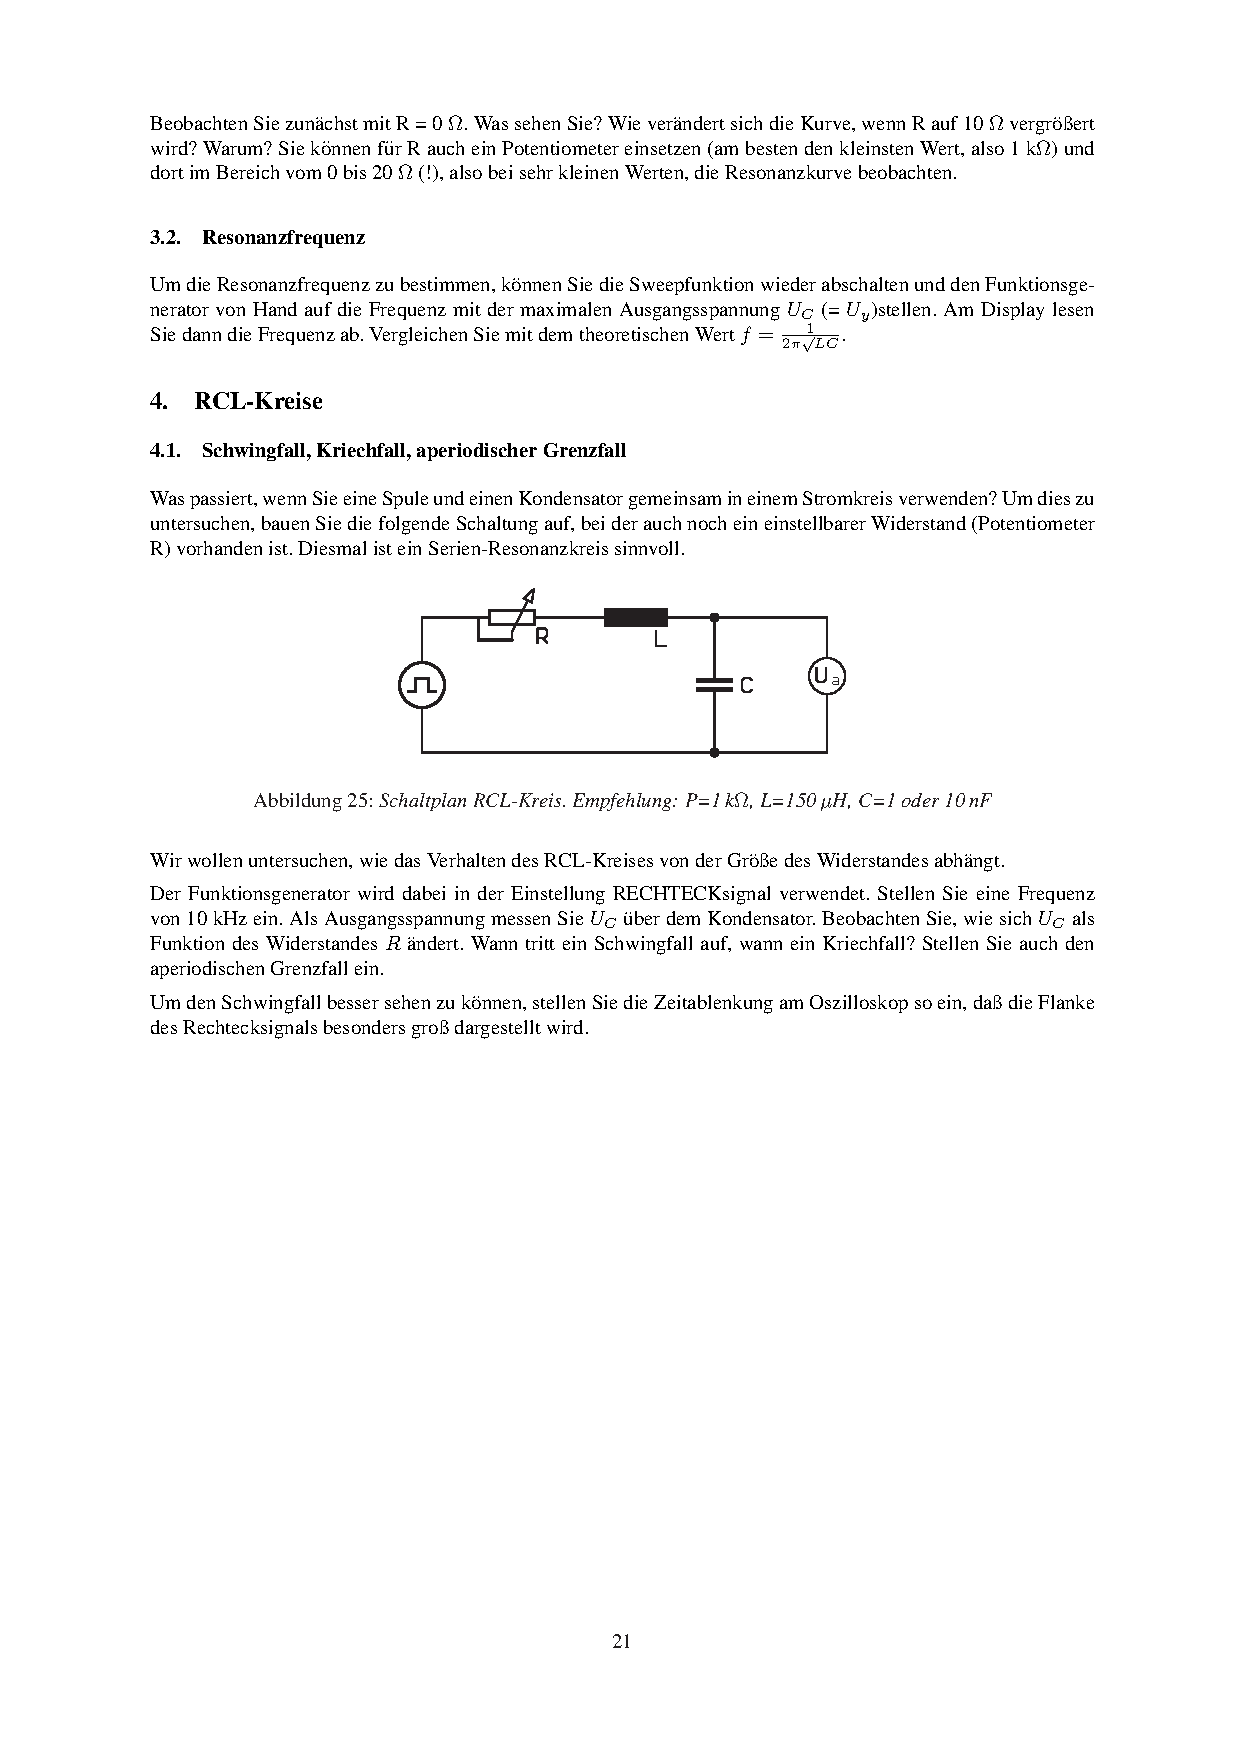
\includegraphics[trim = 20mm 165mm 1mm 95mm, clip, scale = 1]{RCL_kreis.pdf}
  	\caption[Skizze der Schaltung für einen RCL-Kreis, mit Hilfsschaltung]{Skizze der Schaltung für einen RCL-Kreis, mit Hilfsschaltung\footnotemark}
  \label{fig:LC-Kreis_hilfe}
\end{figure}
\footnotetext{Abbildung entnommen von http://www.atlas.uni-wuppertal.de/~kind/E45neu0910.pdf Seite 21 am 22.08.2014}
Wir wollen untersuchen, wie das Verhalten des RCL-Kreises von der Größe des Widerstandes abhängt. Der Funktionsgenerator wird dabei in der Einstellung RECHTECKsignal verwendet. Stellen Sie eine Frequenz von 10 kHz ein. Als Ausgangsspannung messen Sie
$U_C$ über dem Kondensator. Beobachten Sie, wie sich $U_C$
als Funktion des Widerstandes
R ändert. Wann tritt ein Schwingfall auf, wann ein Kriechfall? Stellen Sie auch den
aperiodischen Grenzfall ein. Um den Schwingfall besser sehen zu können, stellen Sie die Zeitablenkung am Oszilloskop so ein, daß die Flanke des Rechtecksignals besonders groß dargestellt wird.
\subsection{Diskussion}
 
\section{Messergebnisse}

\subsection{Aufgabe 2}

\begin{table}[htbp]
\caption{Werte für Aufgabe 2.1.1}
\begin{center}
\begin{tabular}{|l|}
\hline
Widerstand/Ohm \\ \hline
\multicolumn{1}{|r|}{10000 $\pm 500$} \\ \hline
Innenwiderstand/Ohm \\ \hline
\multicolumn{1}{|r|}{10000000} \\ \hline
U$_\text{ein}$/V  \\ \hline
\multicolumn{1}{|r|}{1,0 $(\pm 1)$} \\ \hline
R$_\text{2,L}$/Ohm \\ \hline
\multicolumn{1}{|r|}{9990$(\pm 500)$} \\ \hline
\end{tabular}
\end{center}
\label{tab:2.2.1}
\end{table}

\begin{table}[htbp]
\caption{Werte für Aufgabe 2.1.2}
\begin{center}
\begin{tabular}{|l|}
\hline
Widerstand/Ohm \\ \hline
\multicolumn{1}{|r|}{1000000$(\pm 50000)$} \\ \hline
Innenwiderstand/Ohm  \\ \hline
\multicolumn{1}{|r|}{10000000} \\ \hline
U$_\text{ein}$/V  \\ \hline
\multicolumn{1}{|r|}{1,0 $(\pm 1)$}  \\ \hline
R\_2,L/Ohm \\ \hline
\multicolumn{1}{|r|}{909090 $(\pm 4545)$} \\ \hline
\end{tabular}
\end{center}
\label{tab:2.1.2}
\end{table}


\begin{table}[htbp]
\caption{Werte für Aufgabe 2.2}
\begin{center}
\begin{tabular}{|l|l|}
\hline
Widerstand/Ohm  \\ \hline
\multicolumn{1}{|r|}{1000000 $(\pm 10)$} \\ \hline
Konsensator/F \\ \hline
\multicolumn{1}{|r|}{0,00000010 $(\pm 5)$}\\ \hline
\end{tabular}
\end{center}
\label{tab:2.2}
\end{table}


\begin{table}[htbp]
\caption{Werte für Aufgabe 2.3, für den Frequenzgang}
\begin{center}
\begin{tabular}{|l|l|l|}
\hline
Eingangasfrequenz/Hz & Eingangasfrequenz/Hz & Eingangasfrequenz/Hz \\ \hline
20 $(\pm 10)$ & 50 $(\pm 10)$ & 100 $(\pm 10)$ \\ \hline
U$_\text{aus}$/V & U$_\text{aus}$/V & U$_\text{aus}$/V \\ \hline
4,96 $(\pm 0,05)$ & 4,72 $(\pm 0,05)$ & 4,16 $(\pm 0,05)$ \\ \hline
U$_\text{ein}$/V & U$_\text{ein}$/V & U$_\text{ein}$/V \\ \hline
4,96 $(\pm 0,05)$ & 4,92 $(\pm 0,05)$ & 4,84 $(\pm 0,05)$ \\ \hline \hline
Eingangasfrequenz/Hz & Eingangasfrequenz/Hz & Eingangasfrequenz/Hz \\ \hline
125 $(\pm 10)$ & 150 $(\pm 10)$ & 175 $(\pm 10)$ \\ \hline
U$_\text{aus}$/V & U$_\text{aus}$/V & U$_\text{aus}$/V \\ \hline
3,84 $(\pm 0,05)$ & 3,56 $(\pm 0,05)$ & 3,28 $(\pm 0,05)$ \\ \hline
U$_\text{ein}$/V & U$_\text{ein}$/V & U$_\text{ein}$/V \\ \hline
4,84 $(\pm 0,05)$ & 4,84 $(\pm 0,05)$ & 4,84 $(\pm 0,05)$ \\ \hline \hline
Eingangasfrequenz/Hz & Eingangasfrequenz/Hz & Eingangasfrequenz/Hz \\ \hline 
200 $(\pm 10)$ & 300 $(\pm 10)$ & 400 $(\pm 10)$ \\ \hline
U$_\text{aus}$/V & U$_\text{aus}$/V & U$_\text{aus}$/V \\ \hline
3,04 $(\pm 0,05)$ & 2,28 $(\pm 0,05)$ & 1,8 $(\pm 0,05)$ \\ \hline
U$_\text{ein}$/V & U$_\text{ein}$/V & U$_\text{ein}$/V \\ \hline
4,8 $(\pm 0,05)$ & 4,76 $(\pm 0,05)$ & 4,76 $(\pm 0,05)$ \\ \hline \hline
Eingangasfrequenz/Hz & Eingangasfrequenz/Hz & Eingangasfrequenz/Hz \\ \hline
500 $(\pm 10)$ & 600 $(\pm 10)$ & 700 $(\pm 10)$ \\ \hline
U$_\text{aus}$/V & U$_\text{aus}$/V & U$_\text{aus}$/V \\ \hline
1,5 $(\pm 0,05)$ & 1,24 $(\pm 0,05)$ & 1,08 $(\pm 0,05)$ \\ \hline
U$_\text{ein}$/V & U$_\text{ein}$/V & U$_\text{ein}$/V \\ \hline
4,76 $(\pm 0,05)$ & 4,76 $(\pm 0,05)$ & 4,76 $(\pm 0,05)$ \\ \hline \hline
Eingangasfrequenz/Hz & Eingangasfrequenz/Hz & Eingangasfrequenz/Hz \\ \hline
800 $(\pm 10)$ & 900 $(\pm 10)$ & 1000 $(\pm 10)$ \\ \hline
U$_\text{aus}$/V & U$_\text{aus}$/V & U$_\text{aus}$/V \\ \hline
1 $(\pm 0,05)$ & 0,92 $(\pm 0,05)$ & 0,84 $(\pm 0,05)$ \\ \hline
U$_\text{ein}$/V & U$_\text{ein}$/V & U$_\text{ein}$/V \\ \hline
4,76 $(\pm 0,05)$ & 4,72 $(\pm 0,05)$ & 4,72 $(\pm 0,05)$ \\ \hline \hline
Eingangasfrequenz/Hz & Eingangasfrequenz/Hz &  \\ \hline
75 $(\pm 10)$ & 250 $(\pm 10)$ &  \\ \hline
U$_\text{aus}$/V & U$_\text{aus}$/V &  \\ \hline
4,44 $(\pm 0,05)$ & 2,6 $(\pm 0,05)$ &  \\ \hline
\end{tabular}
\end{center}
\label{tab:2.3}
\end{table}

\begin{table}[htbp]
\caption{Werte für Aufgabe 2.4, zur Bestimmung des Frequenzgangs}
\begin{center}
\begin{tabular}{|l|l|l|}
\hline
Eingangasfrequenz/Hz & Eingangasfrequenz/Hz & Eingangasfrequenz/Hz \\ \hline
850 $(\pm 10)$ & 900 $(\pm 10)$ & 1000 $(\pm 10)$ \\ \hline
U$_aus$/V & U$_aus$/V & U$_aus$/V \\ \hline
3,28 $(\pm 0,05)$ & 3,6 $(\pm 0,05)$ & 4 $(\pm 0,05)$ \\ \hline
U$_\text{ein}$/V & U$_\text{ein}$/V & U$_\text{ein}$/V \\ \hline
6,96 $(\pm 0,05)$ & 7 $(\pm 0,05)$ & 7 $(\pm 0,05)$ \\ \hline \hline
Eingangasfrequenz/Hz & Eingangasfrequenz/Hz & Eingangasfrequenz/Hz \\ \hline
1050 $(\pm 10)$ & 1400 $(\pm 10)$ & 500 $(\pm 10)$ \\ \hline
U$_aus$/V & U$_aus$/V & U$_aus$/V \\ \hline
3,76 $(\pm 0,05)$ & 4,44 $(\pm 0,05)$ & 2,08 $(\pm 0,05)$ \\ \hline
U$_\text{ein}$/V & U$_\text{ein}$/V & U$_\text{ein}$/V \\ \hline
6,88 $(\pm 0,05)$ & 6,8 $(\pm 0,05)$ & 6,96 $(\pm 0,05)$ \\ \hline \hline
Eingangasfrequenz/Hz & Eingangasfrequenz/Hz & Eingangasfrequenz/Hz \\ \hline
650 $(\pm 10)$ & 1700 $(\pm 10)$ & 2000 $(\pm 10)$ \\ \hline
U$_aus$/V & U$_aus$/V & U$_aus$/V \\ \hline
2,6 $(\pm 0,05)$ & 4,7 $(\pm 0,05)$ & 5,3 $(\pm 0,05)$ \\ \hline
U$_\text{ein}$/V & U$_\text{ein}$/V & U$_\text{ein}$/V \\ \hline
6,96 $(\pm 0,05)$ & 6,96 $(\pm 0,05)$ & 6,96 $(\pm 0,05)$ \\ \hline
\end{tabular}
\end{center}
\label{tab:2.4}
\end{table}


\begin{table}[htbp]
\caption{Werte für Aufgabe 2.5, zur Bestimmung des Frequenzgangs}
\begin{center}
\begin{tabular}{|l|l|l|}
\hline
Eingangasfrequenz/Hz & Eingangasfrequenz/Hz & Eingangasfrequenz/Hz \\ \hline
700  $(\pm 10)$ & 900 $(\pm 10)$ & 1000 $(\pm 10)$ \\ \hline
U$_\text{aus}$/V & U$_\text{aus}$/V & U$_\text{aus}$/V \\ \hline
5,08 $(\pm 0,05)$ & 5,16 $(\pm 0,05)$ & 5,2 $(\pm 0,05)$ \\ \hline
U$_\text{ein}$/V & U$_\text{ein}$/V & U$_\text{ein}$/V \\ \hline
5,36 $(\pm 0,05)$ & 5,36 $(\pm 0,05)$ & 5,32 $(\pm 0,05)$ \\ \hline \hline
Eingangasfrequenz/Hz & Eingangasfrequenz/Hz & Eingangasfrequenz/Hz \\ \hline
1200 $(\pm 10)$ & 30000 $(\pm 100)$ & 75000 $(\pm 100)$ \\ \hline
U$_\text{aus}$/V & U$_\text{aus}$/V & U$_\text{aus}$/V \\ \hline
5,2 $(\pm 0,05)$ & 2,36 $(\pm 0,05)$ & 1,08 $(\pm 0,05)$ \\ \hline
U$_\text{ein}$/V & U$_\text{ein}$/V & U$_\text{ein}$/V \\ \hline
5,32 $(\pm 0,05)$ & 5,24 $(\pm 0,05)$ & 5,4 $(\pm 0,05)$ \\ \hline \hline
Eingangasfrequenz/Hz & Eingangasfrequenz/Hz & Eingangasfrequenz/Hz \\ \hline
90000 $(\pm 100)$ & 100000 $(\pm 100)$ & 110000 $(\pm 100)$ \\ \hline
U$_\text{aus}$/V & U$_\text{aus}$/V & U$_\text{aus}$/V \\ \hline
0,928  $(\pm 0,05)$ & 0,840 $(\pm 0,05)$ & 0,776 $(\pm 0,05)$ \\ \hline
U$_\text{ein}$/V & U$_\text{ein}$/V & U$_\text{ein}$/V \\ \hline
5,4 $(\pm 0,05)$ & 5,4 $(\pm 0,05)$ & 5,4 $(\pm 0,05)$ \\ \hline \hline
Eingangasfrequenz/Hz &  &  \\ \hline
12000 $(\pm 100)$ &  &  \\ \hline
U$_\text{aus}$/V &  &  \\ \hline
0,712  $(\pm 0,05)$ &  &  \\ \hline
U$_\text{ein}$/V &  &  \\ \hline
5,4  $(\pm 0,05)$ &  &  \\ \hline
\end{tabular}
\end{center}
\label{tab:2.5}
\end{table}


\begin{table}[htbp]
\caption{Werte für Aufgabe 2.6, zur Bestimmung des Frequenzgangs}
\begin{center}
\begin{tabular}{|l|l|l|}
\hline
Eingangasfrequenz/Hz & Eingangasfrequenz/Hz & Eingangasfrequenz/Hz \\ \hline
1400000 $(\pm 10000)$ & 2000000 $(\pm 10000)$ & 3500000 $(\pm 10000)$ \\ \hline
U$_\text{aus}$/V & U$_\text{aus}$/V & U$_\text{aus}$/V \\ \hline
0,980 $(\pm 0,05)$ & 1,36  $(\pm 0,05)$ & 1,76 $(\pm 0,05)$ \\ \hline
U$_\text{ein}$/V & U$_\text{ein}$/V & U$_\text{ein}$/V \\ \hline
1,58 $(\pm 0,05)$ & 2,16 $(\pm 0,05)$ & 3,34 $(\pm 0,05)$ \\ \hline \hline
Eingangasfrequenz/Hz & Eingangasfrequenz/Hz & Eingangasfrequenz/Hz \\ \hline
4500000 $(\pm 10000)$ & 5000000 $(\pm 10000)$ & 6500000 $(\pm 10000)$ \\ \hline
U$_\text{aus}$/V & U$_\text{aus}$/V & U$_\text{aus}$/V \\ \hline
1,78 $(\pm 0,05)$ & 1,7 $(\pm 0,05)$ & 1,68 $(\pm 0,05)$ \\ \hline
U$_\text{ein}$/V & U$_\text{ein}$/V & U$_\text{ein}$/V \\ \hline
4,00  $(\pm 0,05)$ & 4,22 $(\pm 0,05)$ & 4,44 $(\pm 0,05)$ \\ \hline \hline
Eingangasfrequenz/Hz & Eingangasfrequenz/Hz &  \\ \hline
7500000 $(\pm 10000)$ & 8500000 $(\pm 10000)$ &  \\ \hline
U$_\text{aus}$/V & U$_\text{aus}$/V &  \\ \hline
1,56 $(\pm 0,05)$ & 1,4 $(\pm 0,05)$ &  \\ \hline
U$_\text{ein}$/V & U$_\text{ein}$/V &  \\ \hline
4,58 $(\pm 0,05)$ & 4,58 $(\pm 0,05)$ &  \\ \hline
\end{tabular}
\end{center}
\label{tab:2.6}
\end{table}

\begin{table}[htbp]
\caption{Werte für Aufgabe 3, Materialeigenschaften der Spule und des Kondensators}
\begin{center}
\begin{tabular}{|l|}
\hline
Kondensator/F \\ \hline
0,000001 $(\pm  0,000001)$ \\ \hline
Spule/H \\ \hline
0,00015 $(\pm 0,00008)$ \\ \hline
\end{tabular}
\end{center}
\label{tab:2.6}
\end{table}


\section{Auswertung}

\section{Fazit}
Aufgabe 2 war mit Abstand die längste Aufgabe dieses Versuches und es wurde ein Großteil der verfügbaren Zeit dafür verwendet, was unter anderem daran lag, dass der Anschluss an unseren Funktionsgenerator einen Wackelkontakt hatte, sodass einige Male garnichts angezeigt wurde, obwohl die richtige Schaltung angeschlossen war. Im dritten Aufgabenteil mussten die Messwerte der Nachbargruppe verwendet werden, da wir dort lediglich die Phasenverschiebung ausgemessen haben. Ein großes Problem war auch, dass wir unsere Grenzfrequenzen $\omega_{Gr}$ nicht in die Frequenz f, die am Funktionsgenerator angezeigt wurde, umgerechnet haben. Bei den beiden Hochpässen, sowie beim Bandpass haben wir dadurch den falschen Frequenzbereich ausgemessen, welcher um den Faktor 2$\pi$ größer war, als der eigentlich interessante Frequenzbereich. Insgesamt gab es bei der Durchführung der zweiten Aufgabe also einige Probleme, welche nicht nur auf den semidefekten Anschluss unseres Funktionengenerators zurückzuführen sind, sondern auch auf unseren Fehler bei der Umrechnung von $\omega$ in f\\
Aufgabe 3 verlief dagegen nicht so problematisch, da wir diese an einem anderen Funktionsgenerator durchführen konnten. Bis auf die relativ große Messungenauigkeit beim Ablesen der Resonanzfrequenz am Display liegt unser Ergebnis recht nahe am Theoriewert.\\
Aufgabe 4 veranschaulichte das Verhalten eines RCL Kreises abhängig von der Größe des Widerstandes. Wir haben den Spannungsverlauf am Display eines anderen Frequenzgenerators in allen drei Fällen abfotographiert, wobei uns die Messung des Widerstandes fehlt. Deshalb haben wir die Messerte unserer Nachbargruppe verwendet.\\
Zusammenfassend mussten bei diesem Versuch an einigen Stellen Abstriche gemacht werden. Wir konnten an den meisten Stellen nicht genau genug messen, um qualitative Aussagen zu treffen, da unser Frequenzbereich leider zu groß gewählt war.
%Werte stimmen mit den Formeln überein/nicht überein

\end{document}

